%FOR PDFLATEX USE ONLY
\documentclass[a4paper,12pt]{article}

\usepackage{amssymb,amsmath}

\usepackage[margin=2cm]{geometry}
\usepackage[unicode]{hyperref}
\usepackage[pdftex]{graphicx}
\usepackage{cmlgc}

\usepackage{array}

\usepackage{wrapfig}
\usepackage{array}
\usepackage{lipsum}
\usepackage{esvect}
\usepackage{hyperref}

\usepackage{subfig}
\usepackage{calc}
\usepackage{pgfplots,tikz,circuitikz}
\usepackage{pgfplotstable}
\usepackage{tkz-euclide}

\usepackage{centernot}
\usepackage{cancel}

\usepackage{mathtext}
\usepackage[T1,T2a]{fontenc}
\usepackage[utf8]{inputenc}
\usepackage[english, bulgarian, russian]{babel}
\usepackage{tikz}
\usepackage{pgfplots}
\usepackage[export]{adjustbox}
\usepackage[left=2cm,right=2cm,
    top=2cm,bottom=2cm,bindingoffset=0cm]{geometry}
\usepackage{indentfirst}
\usepackage{braket}
\include{data_40_1}

\begin{document}

\begin{center}
  \LARGE{Работа Д.2.3}\\[0.2cm]
  \LARGE{Определение вязкости воздуха по скорости истечения через капилляр}\\[0.2cm]
  \large{Панферов Андрей}\\[0.2cm]
\end{center}  
  
\section{Аннотация}
В работе производится измерение вязкости воздуха $\eta$ по измерению объёма газа, протекающего через капилляр (иглу шприца) при переменном перепаде давления. Проверяется зависимость расхода газа Q от радиуса капилляра r: $Q \sim r^4$ (формула Пуазейля).
\section{Теоретические сведения}
Вя́зкость (вну́треннее тре́ние) — свойство текучих тел (жидкостей и газов) оказывать сопротивление перемещению одной их части относительно другой. \\
При небольших скоростях газа или жидкости течение среды является ламинарным. Движение среды при этом происходит слоями, обладающими разными скоростями. С увеличением скорости потока движение приобретает сложный, запутанный характер, слои перемешиваются, течение становится турбулентным. При этом скорость в каждой точке быстро меняет величину и направление, сохраняется только её средняя величина.\\
\begin{center}
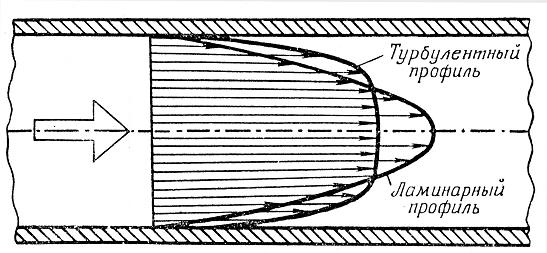
\includegraphics[width=0.3\linewidth]{1.jpg}\\
\end{center}
Характер движения газа или жидкости зависит от соотношения между кинетической энергией движущейся среды и работой сил вязкости. Если первая величина мала по сравнению со второй, то турбулентные пульсации не развиваются и течение остаётся ламинарным. Отношение плотности кинетической энергии к плотности энергетических потерь из-за работы сил вязкости определяет безразмерное число Рейнольдса:
\[ Re = \frac{vr\rho}{\eta} \]
В гладких трубах круглого сечения переход от ламинарного течения к турбулентному происходит при значениях 1000.\\
Для вывода формулы Пуазейля рассмотрим стационарное течение вязкой жидкости или газа по трубе.\\
Мысленно выделим расположенный вдоль оси трубы цилиндр длиной  и радиусом r. Скорость жидкости или газа в разных точках сечения, трубы из-за присутствия силы внутреннего трения различна: она будет наибольшей на оси цилиндра и убывать по мере приближения слоев к стенкам цилиндра, поэтому изменение скорости можно характеризовать градиентом d /dr. С внешней стороны на поверхность выделенного цилиндра действует сила вязкого трения, равная \[ F_{тр} = -\eta\frac{d}{dr}S = -\eta\frac{d}{dr}2\pi rl \]\\
Так как движение жидкости или газа происходит в разных местах трубы с постоянной для этого места скоростью, то сила Fтр должна быть уравновешена силой F давления, вызывающей движение жидкости или газа и создающей перепад давлений $\Delta P = P_1 - P_2$ на торцах выделенного цилиндра, причем эта сила из определения давления равна $S\Delta P$. \\
\[\frac{d}{dr} =  -\frac{\Delta Pr}{2\eta l}\]\\
Постоянная интегрирования получается из граничного условия (скорость у края трубы нулевая), откуда\\
\[v =  \frac{\Delta P}{4\eta l}(R^2-r^2) \]
\[dQ = \frac{dV}{dt} = 2\pi r vdr =2\pi r \frac{\Delta P}{4\eta l}(R^2-r^2)dr \]
\[Q =  \frac{\pi \Delta P r^4}{8\eta l} \]
\section{Метод измерений}
\begin{minipage}{0.45\textwidth} 
Если цилиндр шприца с капилляром погрузить в сосуд с водой, так, как показано на рисунке, то скорость заполнения цилиндра определяется, очевидно, пропускной способностью капилляра, оказывающего наибольшее сопротивление потоку воздуха. По мере заполнения цилиндра перепад давления на длине капилляра изменяется и в момент времени t, показанный на рисунке, равен, очевидно, $P_1 - P_2 = \rho_в gh$, где $\rho_в$– плотность воды.\\
Тогда, в соответствии с формулой Пуазейля, для мгновенного расхода воздуха в момент времени t можно записать: \[ Q = -\frac{Sdh}{dt} = \frac{\pi\rho_вgh_0r^4}{8\eta l}\] \[ ln\frac{h_0}{h} = ln\frac{V_0}{V} = \frac{\pi\rho_вgh_0r^4}{8\eta lS}t\] \[ t =\frac{8\eta lS}{\pi\rho_вgh_0r^4} ln\frac{V_0}{V} = \beta ln\frac{V_0}{V} ]\] \[\eta =  \frac{\pi\rho_вgh_0r^4\beta}{8 lS} \]
\end{minipage}
\begin{minipage}{0.07\textwidth}
\
\end{minipage}
\begin{minipage}{0.45\textwidth}
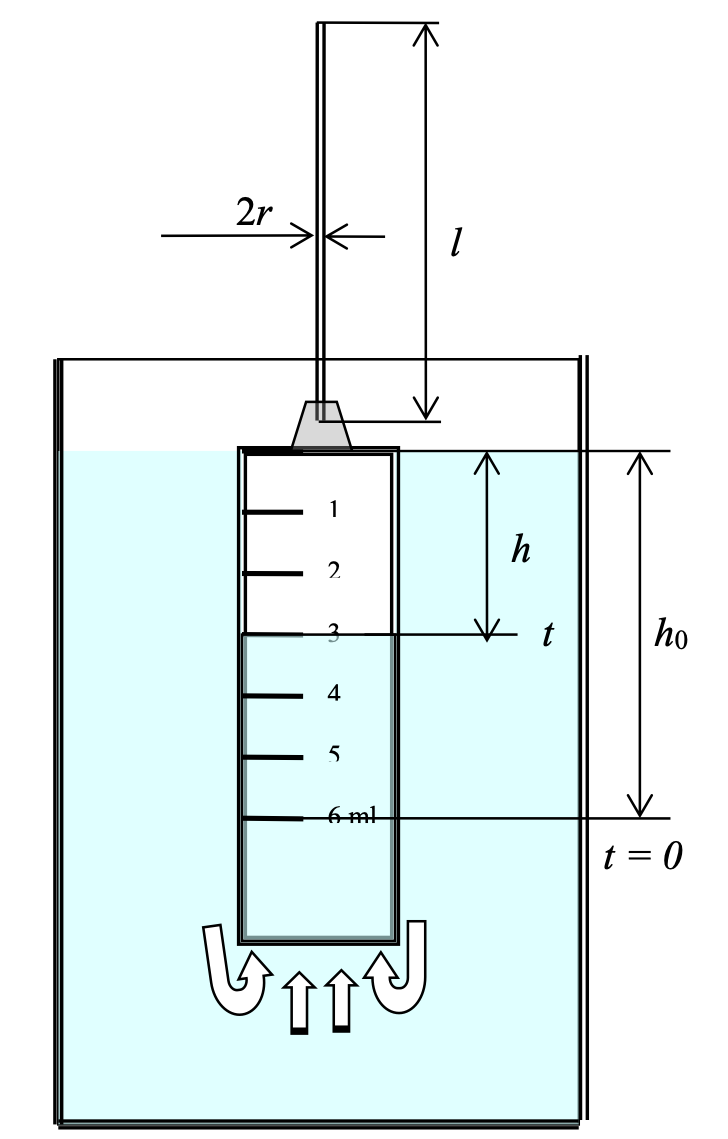
\includegraphics[width=\linewidth]{2.jpg}\\
\end{minipage}
\newpage
\section{Оборудование и инструментальные погрешности}

\textbf{В работе используются:} шприц на 20 мл без поршня (т.е. только цилиндр шприца), сменные капилляры (иглы) разных диаметров d и длин l, секундомер с возможностью фиксации промежуточных значений, прозрачный цилиндрический стакан с водой, линейка, небольшой кусочек ластика.\\

\textbf{Инструментальные погрешности измерений:}\\
\begin{itemize}
\item Обьем шприца -- 0,05 мл
\item Диаметр капилляра -- 0,005 мм
\item Длина капилляра -- 0,5 мм
\item Секундомер -- 0,2 с
\item Линейка -- 0,1 см
\end{itemize}

\section{Результаты измерений и обработка данных}

\subsection{Подготовка к эксперименту}
В аптеке имелось 3 вида шприцов с такими характеристиками иголок:
\begin{center}
\begin{tabular}{|c|c|c|c|c|}
\hline
 $  No   $&тип & $  l, мм $ & $d_{внеш}, мм $ & $ d_{внут}, мм$\\
\hline
     1    & G26  &    12  &   0.45  &   0.26     \\
\hline
    2     &    G23 &30    &   0.60  &   0.34     \\
\hline
    3     & G21  & 38     &  0.80   &    0.51   \\
\hline
\end{tabular}
\end{center}

\subsection{Проведение измерений}


"Длина" шприца -- $7.0 \pm 0.1$см. Используем это для нахождения сечения шприца.\\

Соберем установку согласно схеме и проведем серии экспериментов для каждой иглы. Результаты занесем в соответсвующие таблицы в разделе Данные.\\


После взятия средних значений из каждой выборки пoлучим

\begin{minipage}{0.3\textwidth}
\begin{center}
Измерения для 1 иглы\\
\
\\
\
\\
\
\\

\begin{tabular}{|c|c|c|}
\hline
V, мл&\Delta t, с&$ ln\frac{V_0}{V}$\\
\hline
19 & 4.80 & 0.05 \\
\hline
18 & 9.53 & 0.11 \\
\hline
17 & 14.71 & 0.16 \\
\hline
16 & 19.92 & 0.22 \\
\hline
15 & 25.62 & 0.29 \\
\hline
14 & 31.98 & 0.36 \\
\hline
13 & 38.09 & 0.43 \\
\hline
12 & 45.00 & 0.51 \\
\hline
11 & 52.78 & 0.60 \\
\hline
10 & 61.52 & 0.69 \\
\hline
9 & 69.91 & 0.80 \\
\hline
8 & 80.11 & 0.92 \\
\hline
7 & 91.60 & 1.05 \\
\hline
6 & 104.50 & 1.20\\
\hline
5 & 120.97 & 1.39 \\
\hline
\end{tabular}
\end{center}
\end{minipage}
\begin{minipage}{0.3\textwidth}
\begin{center}
Измерения для 2 иглы\\
\
\\
\begin{tabular}{|c|c|c|}
\hline
V, мл&\Delta t, с& $ln\frac{V_0}{V}$\\
\hline
19 & 1.52 & 0.05 \\
\hline
18 & 3.24 & 0.11 \\
\hline
17 & 5.04 & 0.16 \\
\hline
16 & 6.83 & 0.22 \\
\hline
15 & 8.67 & 0.29 \\
\hline
14 & 10.89 & 0.36 \\
\hline
13 & 13.12 & 0.43 \\
\hline
12 & 15.47 & 0.51 \\
\hline
11 & 18.21 & 0.60 \\
\hline
10 & 21.06 & 0.69 \\
\hline
9 & 24.45 & 0.80 \\
\hline
8 & 27.97 & 0.92 \\
\hline
7 & 32.09 & 1.05 \\
\hline
6 & 36.64 & 1.20 \\
\hline
5 & 42.18 & 1.39 \\
\hline
4 & 49.39 & 1.61 \\
\hline
3 & 58.91 & 1.90 \\
\hline
\end{tabular}
\end{center}
\end{minipage}
\begin{minipage}{0.3\textwidth}
\begin{center}
Измерения для 3 иглы
\begin{tabular}{|c|c|c|}
\hline
V, мл&\Delta t, с&$ ln\frac{V_0}{V}$\\
\hline
19 & 0.54 & 0.05 \\
\hline
18 & 1.12 & 0.11 \\
\hline
17 & 1.77 & 0.16 \\
\hline
16 & 2.42 & 0.22 \\
\hline
15 & 3.01 & 0.29 \\
\hline
14 & 3.77 & 0.36 \\
\hline
13 & 4.55 & 0.43 \\
\hline
12 & 5.36 & 0.51 \\
\hline
11 & 6.21 & 0.60 \\
\hline
10 & 7.07 & 0.69 \\
\hline
9 & 8.16 & 0.80 \\
\hline
8 & 9.42 & 0.92 \\
\hline
7 & 10.77 & 1.05 \\
\hline
6 & 12.43 & 1.20 \\
\hline
5 & 14.11 & 1.39 \\
\hline
4 & 16.50 & 1.61 \\
\hline
3 & 19.30 & 1.90 \\
\hline
2 & 25.14 & 2.30 \\
\hline
\end{tabular}
\end{center}
\end{minipage}
\\
\
\\

$\sigma V \approx 0.5ml $, $ \sigma \Delta t \approx 0.2 с $ \\

Построим графики и найдем их угловые коэффициенты: 


\begin{center}
\begin{tikzpicture}[scale = 1.5]
\begin{axis}[
    legend style={at={(0.97,0.97)}},
    axis lines = left,
    xlabel = {$\Delta t, c$},
    ylabel = {$ln\frac{V_0}{V}$},
    xmin=0, xmax=120,
    ymin=0, ymax=2.5,
	ymajorgrids = true,
	xmajorgrids = true,
	yminorgrids = true, 
	xminorgrids = true, 
	minor tick num = 1 
]

\addplot+[only marks ] plot[error bars/.cd, y dir=both, y explicit]
  coordinates {
	( 4.8 , 0.05129329438755048 )
( 9.529 , 0.10536051565782635 )
( 14.707999999999998 , 0.16251892949777494 )
( 19.916 , 0.22314355131420976 )
( 25.624000000000002 , 0.28768207245178085 )
( 31.982 , 0.3566749439387324 )
( 38.091 , 0.43078291609245434 )
( 44.998 , 0.5108256237659907 )
( 52.778999999999996 , 0.5978370007556204 )
( 61.515 , 0.6931471805599453 )
( 69.912 , 0.7985076962177716 )
( 80.111 , 0.9162907318741551 )
( 91.59599999999999 , 1.0498221244986776 )
( 104.503 , 1.2039728043259361 )
( 120.973 , 1.3862943611198906 )};
	
	
\addplot+[only marks ] plot[error bars/.cd, y dir=both, y explicit]
  coordinates {
	( 1.517 , 0.05129329438755048 )
( 3.243 , 0.10536051565782635 )
( 5.035 , 0.16251892949777494 )
( 6.83 , 0.22314355131420976 )
( 8.668000000000001 , 0.28768207245178085 )
( 10.893999999999998 , 0.3566749439387324 )
( 13.115 , 0.43078291609245434 )
( 15.469000000000003 , 0.5108256237659907 )
( 18.213 , 0.5978370007556204 )
( 21.057000000000002 , 0.6931471805599453 )
( 24.445999999999994 , 0.7985076962177716 )
( 27.965000000000003 , 0.9162907318741551 )
( 32.095 , 1.0498221244986776 )
( 36.644999999999996 , 1.2039728043259361 )
( 42.178000000000004 , 1.3862943611198906 )
( 49.391999999999996 , 1.6094379124341003 )
( 58.913 , 1.8971199848858813 )};


\addplot+[only marks ] plot[error bars/.cd, y dir=both, y explicit]
  coordinates {
	( 0.537 , 0.05129329438755048 )
( 1.117 , 0.10536051565782635 )
( 1.7710000000000001 , 0.16251892949777494 )
( 2.425 , 0.22314355131420976 )
( 3.006 , 0.28768207245178085 )
( 3.7689999999999997 , 0.3566749439387324 )
( 4.553000000000001 , 0.43078291609245434 )
( 5.355000000000001 , 0.5108256237659907 )
( 6.2090000000000005 , 0.5978370007556204 )
( 7.071000000000001 , 0.6931471805599453 )
( 8.157999999999998 , 0.7985076962177716 )
( 9.415000000000001 , 0.9162907318741551 )
( 10.769000000000002 , 1.0498221244986776 )
( 12.426000000000002 , 1.2039728043259361 )
( 14.109 , 1.3862943611198906 )
( 16.5 , 1.6094379124341003 )
( 19.304000000000002 , 1.8971199848858813 )
( 25.144000000000002 , 2.302585092994046 )};

\addplot+[brown] coordinates{(  -1,-0.09506791102833415 ) ( 100, 9.506791102833415)};	
\addplot+[red] coordinates{(  -1,-0.03245965861405302) ( 100, 3.245965861405302)};	
\addplot+[blue] coordinates{(  -1,-0.01153072017039334 ) ( 1000, 11.53072017039334)};	

	
\legend{ 
	1 шприц\\
	2 шприц\\
	3 шприц\\
	};

\end{axis}
\end{tikzpicture}
\end{center}
\\
\newpage
Из графиков можно получить значения наклонов прямых, $\beta$, а так же из табличных данных оценить среднюю скорость по расходу, откуда пересчитать число Рейнольдса и характерное расстояние ($l_{хар} \approx 0.2\cdot r\cdot Re$):\\

\begin{center}
\begin{tabular}{|c|c|c|c|c|c|}
\hline
 $  No   &$\beta, c^{-1}$ &\eta, Па \cdot c \cdot 10^{-5} & $v, \frac{мм}{c}$& Re & l_{хар}, мм \\
\hline
     1    & 86.7   & 1.95 &0.4& 2.66& 0.14\\
\hline
    2     &    30.8  &  1.81 &1.2&10.27&0.70 \\
\hline
    3     & 10.5    & 1.11 &3.6&82.70& 8.4\\
\hline
\end{tabular}
\end{center}

\[ \eta_{ср} = (1.62 \pm 0.23) \cdot 10^{-5} Па\cdot c\]

Сравнивая с табличным:

\[\eta_{табл} = 1.78 \cdot 10^{-5} Па\cdot c\]


 \section{Выводы и рассчёт погрешностей}
 \subsection{Погрешности}
 \begin{equation*}
\frac{\Delta \eta}{\eta} = \sqrt{\frac{1}{N^2}\sum\limits_1^n{((\frac{\Delta t}{t})^2+(\frac{\Delta V}{V})^2})+(\frac{\Delta L}{L})^2+(\frac{\Delta h}{h})^2+(\frac{\Delta S}{S})^2+16(\frac{\Delta r}{r})^2+\sigma_{эксп}^2} \approx 14\%\\
\end{equation*}
 \subsection{Вывод}
 В результате эксперимента было получено значение коэффициента вязкости воздуха, проведена оценка чисел Рейнольдса для каждой серии опытов, а так же была проведена оценка характерных расстояний, при которых устанавливается ламинарное течение. Теоретическая зависимость совпадает с экспериментальной, совпадение значений друг с другом не только по порядку, но ещё и с табличным значением в пределах погрешности ($1.78 \cdot 10^{-5} Па\cdot c$) говорит о том, что примененная модель течения газа хорошо описывает наблюдаемый процесс. Случайная погрешность данных оказалась относительн малой в сравнении с другими погрешностями(меньше 2 процентов), что значит, можно было бы обойтись 3 сериями измерений с каждой иглой. Проведения измерений с углекислым газом не были произведены так как не удалось приобрести необходимое оборудование - резиновые шарики (в шарик засыпается сода и уксус в пропорции 1:2, далее происходит реакция, в шарике находится почти чистый углекислый газ, этим газом можно продувать и наполнять шприц так, чтобы потом опустить в воду и под действием разности давлений воды СО2 выходил наружу). 

 \newpage

 \begin{center}
Измерения для 1 шприца
\begin{tabular}{|c|c|c|c|c|c|c|c|c|c|c|}
\hline
V (мл)&\Delta t_1 (с)&\Delta t_2 (с)&\Delta t_3 (с)&\Delta t_4 (с)&\Delta t_5 (с)&\Delta t_6 (с)&\Delta t_7 (с)&\Delta t_8 (с)&\Delta t_9 (с)&\Delta t_{10} (с)\\
\hline
19.0 & 6.00 & 4.14 & 5.06 & 4.65 & 4.12 & 4.6 & 5.1 & 4.91 & 4.40 & 5.02 \\
\hline
18.0 & 12.70 & 8.42 & 9.29 & 8.82 & 8.09 & 10.25 & 9.33 & 10.03 & 8.58 & 9.78 \\
\hline
17.0 & 18.82 & 13.58 & 13.71 & 13.48 & 13.29 & 14.86 & 15.25 & 15.02 & 13.98 & 15.09 \\
\hline
16.0 & 24.65 & 18.74 & 18.35 & 18.41 & 18.08 & 19.94 & 20.72 & 19.31 & 19.99 & 20.97 \\
\hline
15.0 & 31.56 & 24.34 & 24.51 & 23.46 & 22.91 & 26.10 & 27.02 & 25.12 & 24.79 & 26.43 \\
\hline
14.0 & 39.02 & 30.13 & 30.83 & 28.83 & 28.20 & 32.21 & 33.37 & 31.12 & 31.97 & 34.14 \\
\hline
13.0 & 46.48 & 36.17 & 37.46 & 34.26 & 34.23 & 38.44 & 40.48 & 36.3 & 36.65 & 40.44 \\
\hline
12.0 & 55.48 & 42.65 & 43.26 & 40.09 & 39.90 & 45.56 & 47.53 & 43.77 & 43.45 & 48.29 \\
\hline
11.0 & 64.64 & 49.69 & 51.42 & 46.81 & 46.79 & 54.59 & 56.56 & 51.33 & 50.66 & 55.30 \\
\hline
10.0 & 74.66 & 57.29 & 60.83 & 54.20 & 53.51 & 62.20 & 66.13 & 60.36 & 60.74 & 65.23 \\
\hline
9.0 & 85.57 & 65.01 & 68.39 & 61.83 & 60.58 & 70.95 & 76.74 & 68.21 & 67.46 & 74.38 \\
\hline
8.0 & 97.79 & 73.94 & 79.64 & 70.34 & 67.30 & 81.28 & 87.92 & 79.03 & 78.15 & 85.72 \\
\hline
7.0 & 110.86 & 84.85 & 93.73 & 79.86 & 76.37 & 91.78 & 100.81 & 90.81 & 87.29 & 99.6 \\
\hline
6.0 & 126.90 & 97.10 & 107.14 & 90.52 & 85.66 & 103.77 & 115.21 & 105.57 & 99.15 & 114.01 \\
\hline
5.0 & 147.00 & 107.44 & 124.24 & 102.39 & 98.21 & 121.38 & 130.47 & 130.39 & 114.65 & 133.56 \\
\hline
\end{tabular}
\end{center}

\begin{center}
Измерения для 2 шприца
\begin{tabular}{|c|c|c|c|c|c|c|c|c|c|c|}
\hline
V (мл)&\Delta t_1 (с)&\Delta t_2 (с)&\Delta t_3 (с)&\Delta t_4 (с)&\Delta t_5 (с)&\Delta t_6 (с)&\Delta t_7 (с)&\Delta t_8 (с)&\Delta t_9 (с)&\Delta t_{10} (с)\\
\hline
19.0 & 1.86 & 1.36 & 1.64 & 1.50 & 1.38 & 1.44 & 1.21 & 1.70 & 1.43 & 1.65 \\
\hline
18.0 & 3.64 & 3.05 & 3.20 & 3.25 & 2.69 & 3.27 & 3.47 & 3.37 & 3.30 & 3.19 \\
\hline
17.0 & 5.78 & 4.88 & 5.23 & 4.92 & 4.81 & 4.83 & 5.13 & 5.10 & 5.02 & 4.65 \\
\hline
16.0 & 7.50 & 6.76 & 7.08 & 6.82 & 6.62 & 6.75 & 6.76 & 6.65 & 6.88 & 6.48 \\
\hline
15.0 & 9.01 & 8.52 & 8.98 & 8.48 & 8.52 & 8.51 & 8.61 & 8.66 & 8.69 & 8.70 \\
\hline
14.0 & 11.43 & 10.82 & 11.22 & 10.58 & 10.27 & 10.97 & 10.85 & 11.12 & 11.02 & 10.66 \\
\hline
13.0 & 13.77 & 13.15 & 13.34 & 12.83 & 12.60 & 13.41 & 13.18 & 12.87 & 13.14 & 12.86 \\
\hline
12.0 & 16.05 & 15.14 & 15.75 & 15.34 & 14.87 & 15.73 & 15.86 & 15.31 & 15.65 & 14.99 \\
\hline
11.0 & 19.28 & 17.84 & 18.57 & 17.90 & 17.25 & 18.37 & 18.46 & 18.01 & 18.83 & 17.62 \\
\hline
10.0 & 22.55 & 20.58 & 21.57 & 21.05 & 20.51 & 21.50 & 20.22 & 20.99 & 21.14 & 20.46 \\
\hline
9.0 & 26.01 & 24.28 & 24.78 & 24.02 & 23.38 & 24.76 & 24.76 & 24.26 & 24.82 & 23.39 \\
\hline
8.0 & 30.01 & 27.78 & 28.19 & 27.45 & 26.43 & 27.98 & 28.22 & 28.05 & 28.56 & 26.98 \\
\hline
7.0 & 34.34 & 31.14 & 32.32 & 31.34 & 30.97 & 32.45 & 32.27 & 32.72 & 32.46 & 30.94 \\
\hline
6.0 & 39.17 & 36.05 & 37.76 & 36.77 & 35.39 & 37.05 & 37.18 & 36.08 & 36.24 & 34.76 \\
\hline
5.0 & 46.20 & 41.19 & 42.11 & 41.63 & 40.35 & 42.78 & 41.84 & 42.24 & 42.57 & 40.87 \\
\hline
4.0 & 55.48 & 48.02 & 49.47 & 49.16 & 47.72 & 49.61 & 48.34 & 49.39 & 49.34 & 47.39 \\
\hline
3.0 & 65.70 & 56.84 & 57.78 & 60.21 & 57.18 & 59.44 & 56.94 & 59.35 & 59.19 & 56.50 \\
\hline\end{tabular}
\end{center}

\begin{center}
Измерения для 3 шприца
\begin{tabular}{|c|c|c|c|c|c|c|c|c|c|c|}
\hline
V (мл)&\Delta t_1 (с)&\Delta t_2 (с)&\Delta t_3 (с)&\Delta t_4 (с)&\Delta t_5 (с)&\Delta t_6 (с)&\Delta t_7 (с)&\Delta t_8 (с)&\Delta t_9 (с)&\Delta t_{10} (с)\\
\hline
19.0 & 0.50 & 0.45 & 0.63 & 0.72 & 0.61 & 0.56 & 0.44 & 0.43 & 0.53 & 0.50 \\
\hline
18.0 & 1.00 & 0.91 & 1.36 & 1.56 & 1.16 & 1.09 & 0.87 & 1.05 & 1.11 & 1.06 \\
\hline
17.0 & 1.66 & 1.37 & 2.15 & 2.25 & 1.63 & 1.81 & 1.49 & 1.65 & 1.95 & 1.75 \\
\hline
16.0 & 2.14 & 2.03 & 2.84 & 2.85 & 2.49 & 2.38 & 2.25 & 2.32 & 2.61 & 2.34 \\
\hline
15.0 & 2.67 & 2.60 & 3.41 & 3.54 & 3.07 & 2.91 & 2.71 & 3.00 & 3.29 & 2.86 \\
\hline
14.0 & 3.74 & 3.49 & 4.17 & 4.15 & 3.83 & 3.66 & 3.42 & 3.74 & 3.83 & 3.66 \\
\hline
13.0 & 4.72 & 4.31 & 4.92 & 5.00 & 4.79 & 4.37 & 4.12 & 4.46 & 4.42 & 4.42 \\
\hline
12.0 & 5.36 & 5.04 & 5.62 & 5.91 & 5.40 & 5.03 & 5.30 & 5.39 & 5.27 & 5.23 \\
\hline
11.0 & 6.31 & 5.77 & 6.79 & 6.71 & 6.10 & 5.99 & 5.97 & 6.15 & 6.28 & 6.02 \\
\hline
10.0 & 7.20 & 6.68 & 7.45 & 8.14 & 7.06 & 6.84 & 6.52 & 6.85 & 7.03 & 6.94 \\
\hline
9.0 & 8.21 & 8.16 & 8.61 & 9.12 & 8.58 & 7.58 & 7.58 & 7.79 & 8.10 & 7.85 \\
\hline
8.0 & 9.41 & 9.33 & 10.09 & 10.61 & 9.39 & 9.10 & 8.91 & 8.89 & 9.29 & 9.13 \\
\hline
7.0 & 11.23 & 10.93 & 11.80 & 11.77 & 10.75 & 10.26 & 10.07 & 10.05 & 10.54 & 10.29 \\
\hline
6.0 & 13.02 & 12.26 & 13.51 & 13.40 & 12.56 & 11.57 & 12.11 & 11.44 & 12.17 & 12.22 \\
\hline
5.0 & 14.38 & 14.44 & 14.94 & 15.04 & 14.32 & 12.83 & 13.34 & 14.22 & 13.40 & 14.18 \\
\hline
4.0 & 15.98 & 16.94 & 17.78 & 17.16 & 16.36 & 16.15 & 16.29 & 15.09 & 16.67 & 16.58 \\
\hline
3.0 & 19.04 & 19.21 & 20.38 & 20.36 & 18.61 & 19.02 & 19.62 & 18.07 & 19.49 & 19.24 \\
\hline
2.0 & 24.17 & 28.53 & 26.04 & 27.17 & 22.67 & 23.08 & 27.85 & 22.58 & 24.90 & 24.45 \\
\hline
\end{tabular}
\end{center}
 \end{document}
